\documentclass[12pt,a4paper]{article}
\usepackage{amsmath,amscd,amsbsy,amssymb,latexsym,url,bm,amsthm}
\usepackage{epsfig,graphicx,subfigure}
\usepackage{enumitem,balance}
\usepackage{wrapfig}
\usepackage{mathrsfs,euscript}
\usepackage[usenames]{xcolor}
\usepackage{hyperref}
\usepackage[vlined,ruled,linesnumbered]{algorithm2e}
\usepackage{float}
\usepackage{cite}
\usepackage{booktabs}
\usepackage{listings}
\usepackage{xcolor}
\lstset{
    language=Python,
    basicstyle=\ttfamily,
    keywordstyle=\color{blue}\ttfamily,
    stringstyle=\color{red}\ttfamily,
    commentstyle=\color{brown}\ttfamily,
    morecomment=[l][\color{magenta}]{\#},
    numbers=left,
    numberstyle=\tiny\color{gray},
    numbersep=5pt,
    showspaces=false,
    showstringspaces=false,
    frame=single
}
\hypersetup{colorlinks=true,linkcolor=black}

\newtheorem{theorem}{Theorem}
\newtheorem{lemma}[theorem]{Lemma}
\newtheorem{proposition}[theorem]{Proposition}
\newtheorem{corollary}[theorem]{Corollary}
\newtheorem{exercise}{Exercise}
\newtheorem*{solution}{Solution}
\newtheorem{definition}{Definition}
\theoremstyle{definition}

\renewcommand{\thefootnote}{\fnsymbol{footnote}}

\newcommand{\postscript}[2]
 {\setlength{\epsfxsize}{#2\hsize}
  \centerline{\epsfbox{#1}}}

\renewcommand{\baselinestretch}{1.0}

\setlength{\oddsidemargin}{-0.365in}
\setlength{\evensidemargin}{-0.365in}
\setlength{\topmargin}{-0.3in}
\setlength{\headheight}{0in}
\setlength{\headsep}{0in}
\setlength{\textheight}{10.1in}
\setlength{\textwidth}{7in}
\makeatletter \renewenvironment{proof}[1][Proof] {\par\pushQED{\qed}\normalfont\topsep6\p@\@plus6\p@\relax\trivlist\item[\hskip\labelsep\bfseries#1\@addpunct{.}]\ignorespaces}{\popQED\endtrivlist\@endpefalse} \makeatother
\makeatletter
\renewenvironment{solution}[1][Solution] {\par\pushQED{\qed}\normalfont\topsep6\p@\@plus6\p@\relax\trivlist\item[\hskip\labelsep\bfseries#1\@addpunct{.}]\ignorespaces}{\popQED\endtrivlist\@endpefalse} \makeatother
\setlength{\parindent}{0pt}
\bibliographystyle{acm}

\begin{document}
\title{\textbf{Homework 2}}
\author{Zhengxiang Huang}
\date{520021910014}
\maketitle

\tableofcontents
\newpage

\section{Introduction}
In this Homework, you shall yourself explore more on how to implement quantization, 
and deploy LLM on Nano with the multiple online resources. 

We sincerely hope you enjoy your journey through this homework as we do. Have fun!

\section{Q1: Quantization in PyTorch (85')}


\subsection{Problem Formulation}
We've discussed quantization in class. 

Now, try to quantize your own network in Homework 1 Q5 on your own laptop computer.

You shall then be able to answer the following questions:

\begin{enumerate}
    \item (5') Q: Screenshot the results of "print(qconfig)". Explain the parameters of it. e.g., explain what is "per\_channel\_symmetric".

    \item (10') Q: Implement "fuse\_model" function for your model, explain how "Conv2d", "BatchNorm2d", and "ReLU" are fused. Screenshot the results of "print(model)" after you fuse it.

    \item (10') Q: Calibrate and quantize your model in PyTorch. Screenshot the results of "print(model)" after you quantize it. Explain why we need calibration phase, and what we are observing during that phase.

    \item (20') Q: Measure the size, inference accuracy, and inference time of your model after quantization. Compare the size, time, and accuracy before and after quantization.

    \item (40') Q: Submit your quantization code, whether it's runnable or not. (Even it can't work, we attribute some points to you.)
    
    \item (Bonus +15') Q: Quantized model can't be directly deployed on nano, we need onnx workaround. We have a line of "torch.onnx.export" in our "example.py". Search online how to install and run the "quant.onnx" you export, and deploy that stuff onto your Nano board with onnx. If onnx is impossible on nano, write in the report to inform me, and I will attributes bouns to you too. (No hints nor guides, search yourself! hahahaha!)

    
\end{enumerate}

(\textbf{Hint}: It's suggested that you install a CPU version of Pytorch on your own computer if you don't have a powerful Nvidia GPU installed. 

"pip install torch==2.0.1 torchvision==0.15.2 --index-url https://download.pytorch.org/whl/cpu" to install a cpu version pytorch on your computer, if you previously have no pytorch installed.)

(\textbf{Hint}: Refer to \href{PyTorch PTSQ}{https://pytorch.org/docs/stable/quantization.html\#post-training-static-quantization} and \href{PyTorch PTSQ for MBNet}{https://pytorch.org/tutorials/advanced/static\_quantization\_tutorial.html} for more information of how to quantize a model in PyTorch. Also, see our "example.py" and "model.py" provided.)

\subsection{Solution}
(Your answers go here!)




\section{Q2: Advanced Topic, LLM on Nano (15')}
\subsection{Problem Formulation}
\begin{enumerate}
    \item (12') Follow our instructions in LLM-README.md to deploy a LLM (Qwen1.5-4B) on Nano. Measure time and space it consumes. Have fun chatting with it! Screenshot your conversions.
    
    \begin{figure}[H]
        \centering
        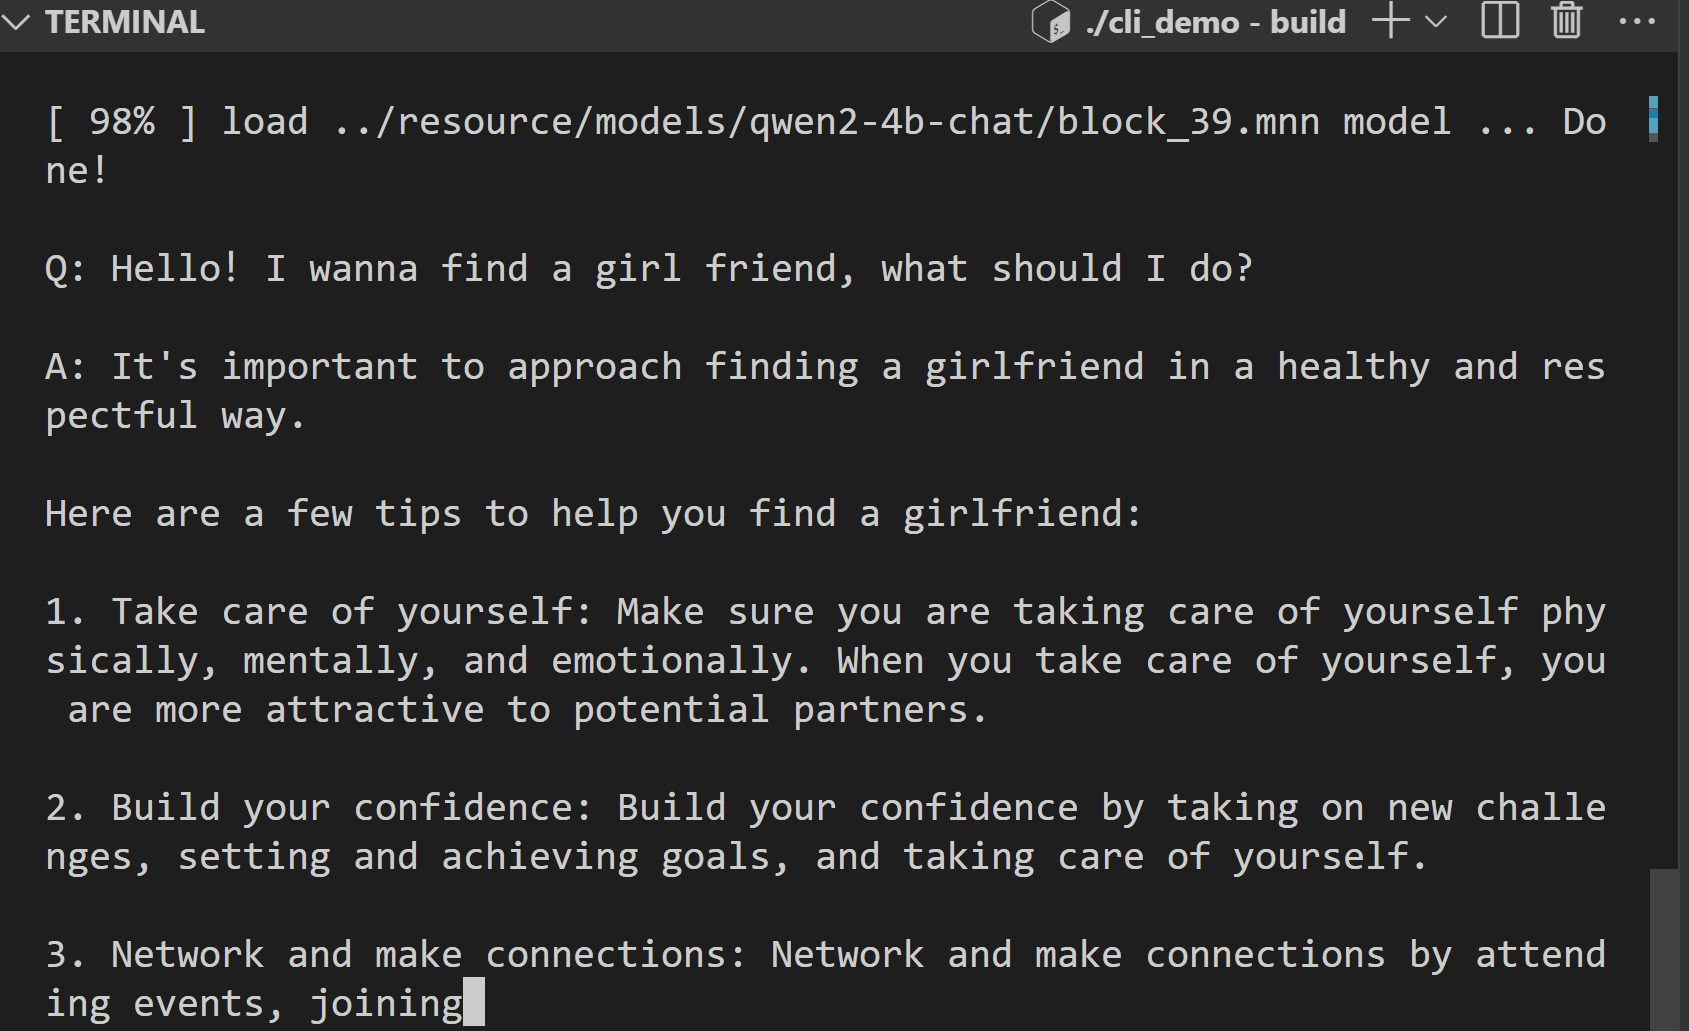
\includegraphics[width=0.7\textwidth]{qwen-llm.jpg}
        \caption{Nano Chat Bot}
        \label{fig:enter-label}
    \end{figure}
    
    The resource LLM takes up.
    
    \begin{figure}[H]
        \centering
        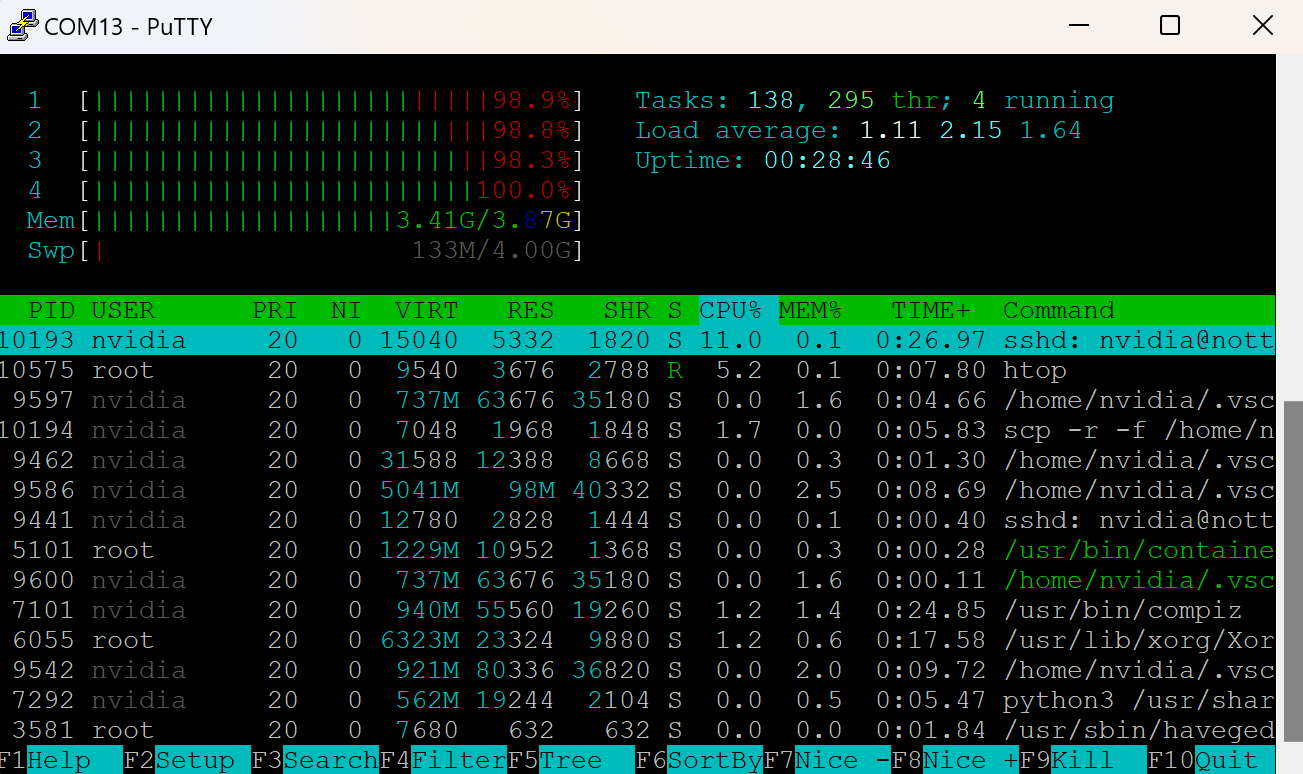
\includegraphics[width=0.7\textwidth]{llm-resource.jpg}
        \caption{LLM resource}
        \label{fig:enter-label}
    \end{figure}
    
    (Hint: If you can't deploy it, screenshot the step you get stuck and we will attribute points to you!)

    \item (3') Tell me how many bit are this model's weights quantized into? 4 bits? 8 bits? No quantization? Where did you find that info?
    
\end{enumerate}




\subsection{Solution}
(Your answer here!)

\section{What have you learned?}
\subsection{Problem Formulation}
(Your answer here!)

\subsection{Tell me what you have learned}
(Your answer here!)

\section{Acknowledgement}
(Your answer here!)



\bibliography{ref}
\end{document}